%%%%%%%%%%%%%%%%%%%%%%%%%%%%%%%%%%%%%%%%%%%%%%%%%%%%%%%%%%%%%%%%%%%%%%%%%%%%%%%%
%2345678901234567890123456789012345678901234567890123456789012345678901234567890
%        1         2         3         4         5         6         7         8
\documentclass[letterpaper, 10 pt, conference]{ieeeconf}  % Comment this line out
                                                          % if you need a4paper
%\documentclass[a4paper, 10pt, conference]{ieeeconf}      % Use this line for a4
                                                          % paper

\IEEEoverridecommandlockouts                              % This command is only
                                                          % needed if you want to
                                                          % use the \thanks command
\overrideIEEEmargins
% See the \addtolength command later in the file to balance the column lengths
% on the last page of the document
% The following packages can be found on http:\\www.ctan.org
%\usepackage{graphics} % for pdf, bitmapped graphics files
%\usepackage{epsfig} % for postscript graphics files
%\usepackage{mathptmx} % assumes new font selection scheme installed
%\usepackage{times} % assumes new font selection scheme installed
%\usepackage{amsmath} % assumes amsmath package installed
%\usepackage{amssymb}  % assumes amsmath package installed

\title{\LARGE \bf
Optimal Data Intensive Flows for Network on Chip Mesh Networks
}
%\author{ \parbox{3 in}{\centering Huibert Kwakernaak*
%         \thanks{*Use the $\backslash$thanks command to put information here}\\
%         Faculty of Electrical Engineering, Mathematics and Computer Science\\
%         University of Twente\\
%         7500 AE Enschede, The Netherlands\\
%         {\tt\small h.kwakernaak@autsubmit.com}}
%         \hspace*{ 0.5 in}
%         \parbox{3 in}{ \centering Pradeep Misra**
%         \thanks{**The footnote marks may be inserted manually}\\
%        Department of Electrical Engineering \\
%         Wright State University\\
%         Dayton, OH 45435, USA\\
%         {\tt\small pmisra@cs.wright.edu}}
%}

\author{Junwei Zhang$^{1}$ Esther Arkin$^{1}$ and Thomas Robertazzi$^{2}$% <-this % stops a space
\thanks{}% <-this % stops a space
\thanks{$^{1}$Junwei Zhang, Ph.D. candidate of Applied Mathematics and Statistics department,
        Stony Brook University, stony brook, NY 11794
        {\tt\small junwei.zhang@stonybrook.edu}}%  
\thanks{$^{1}$Esther Arkin, Professor of Applied Mathematics and Statistics department, Stony Brook University,
        stony brook, NY 11794
        {\tt\small esther.arkin@stonybrook.edu}}%
\thanks{$^{2}$Thomas Robertazzi, Professor of Electrical and Computer Engineering department, Stony Brook University,
        stony brook, NY 11794
        {\tt\small Thomas.Robertazzi@stonybrook.edu}}%
}
\usepackage[utf8]{inputenc}
\usepackage[english]{babel} 
\usepackage{biblatex}
\usepackage{graphicx}		% to see postscript files
\usepackage{empheq}
\usepackage{mathtools}
\usepackage{caption}
\usepackage[dvips]{epsfig}
\usepackage{multirow}
\usepackage{color}
\usepackage{listings}
\usepackage{verbatim}
\usepackage{epstopdf}
\usepackage{subcaption}
\usepackage{mathrsfs}
\usepackage{algorithm}
\usepackage{algorithmic}
\usepackage{url}
\usepackage{amsmath,empheq}
\usepackage[utf8]{inputenc}
\usepackage[english]{babel}

\addbibresource{references.bib}

\begin{document}

\maketitle
\thispagestyle{empty}
\pagestyle{empty}

%%%%%%%%%%%%%%%%%%%%%%%%%%%%%%%%%%%%%%%%%%%%%%%%%%%%%%%%%%%%%%%%%%%%%%%%%%%%%%%%
\begin{abstract}
Abstract Here

{\it Key Words:}


\end{abstract}

%%%%%%%%%%%%%%%%%%%%%%%%%%%%%%%%%%%%%%%%%%%%%%%%%%%%%%%%%%%%%%%%%%%%%%%%%%%%%%%%
\section{INTRODUCTION}

\subsection{Related Literature}

\subsubsection{Divisible Load Theory}
Crucial to our success in the single and multiple injection point cases, is the use of divisible load scheduling theory [refs].  Developed over the past few decades, it assumes load is a continuous variable that can be arbitrarily partitioned among processors and links in a network.  Use is made of the divisible load scheduling’s optimality principle [ref], which say makespan is minimized when one forces all processors to stop at the same time (intuitively otherwise one could transfer load from busy to idle processors to achieve a better solution).  This leads to a series of chained linear flow and processing equations that can be solved by linear equation techniques, often yielding recursive and even closed form solutions for quantities such as makespan and speedup. 

\subsubsection{Voronoi Diagrams}
In the context of multiple injection point models, this paper represents 
Jia  \cite{jia2010scheduling} proposes a genetic algorithm, which utilize a novel Graph Partitioning (GP) scheme to partition the network such that each source in the network gains a portion of network resources and then these sources cooperate to process their loads.  We utilize the Voronoi diagrams \cite{jia2010scheduling} in conjunction with divisible load scheduling for a significant applied problem. 

In mathematics, a Voronoi diagram \cite{fortune1995voronoi} a partitioning of a plane into regions based on distance to points in a specific subset of the plane. For each seed there is a corresponding region consisting of all points closer to that seed than to any other. These regions are called Voronoi cells. 

\subsection{Problem Description}
Networks on chips (NOC) represent the smallest networks that have been implemented to date \cite{robertazzi2017computer}.  A popular choice for the interconnection network on such networks on chips is the rectangular mesh.  It is straightforward to implement and is a natural choice for a planar chip layout.

Data to be processed can be inserted into the chip at one or more so-called “injection points”, that is node(s) in the mesh that forward the data to other nodes.  Beyond NOCs, injecting data into a parallel processor’s interconnection network has been done for some time, notably in IBM’s Bluegene machines \cite{krevat2002job}.  In this paper it is sought to determine, for a given set of injection points how, optimally or near-optimally, to assign load to different processors in a known timed pattern so as to process a load of data in a minimal amount of time (i.e. minimize makespan).  In this paper we succeed in presenting an optimal technique for single injection points in homogeneous meshes that involves no more complexity than linear equation solution.  For multiple injection points we present algorithms that produce near optimal solutions using Voronoi diagrams \cite{fortune1987sweepline} \cite{jia2010scheduling}.  The methodology presented here can be applied to a variety of switching/scheduling protocols besides those directly covered in this paper. 

In this paper, we investigate the virtual cut-through switching \cite{kermani1979virtual}.  In the virtual cut-through environment, a node can begin relaying the first part of a message (packet) along a transmission path as soon as it starts to arrive at the node , that is, it doesn't have to wait to receive the entire message before it can begin forwarding the message.

Equivalence computation \cite{robertazzi1993processor} is a technique, which consists of combining a cluster of processors as one whole equivalent processor to process a unit $1$ workload.

\section{Assumption and Notion}

\subsection{Assumption}
The following assumptions are used throughout the paper:

\begin{itemize}
\item Under virtual cut-through switching, a node can relay the beginning bit of a message (packet) before the entire message is received. 
\item For simplicity, return communication is not considered.  
\item The communication delays are taken into consideration.  
\item The time costs of computation and communication are assumed to be linear function of the data size.  
\item The network environment is homogeneous, that is, all the processors have the same computation capacity.  The link speeds between any two unit cores are identical.   
\item The number of outgoing ports in each processor is limited.  In NOC (network on chip), the port number is fixed 4 or 5  \cite{robertazzi2017computer}.    
\item Single Path Communication : data transfer between two nodes follows a single path
\item Homogeneous : a homogeneous (all link and processors speed are identical ) is assumed.
\item Equivalence computation : the problem's objective function is how to partition and schedule the workloads amongst the processors to obtain the minimum makespan (finish time).  
\item Multi-source assignment : how all processors can finish processing a unit $1$ workload at the same time utilizing fewer processors.
\end{itemize}

\subsection{Notions}
The following notations and definitions are utilized:
\begin{itemize}
\item $P_{i}$: The $i$th processor.   $0  \leq i \leq m*n-1$.  
\item $L_{i}$: The $i$th work load.   $1 \leq i \leq k$.  
\item $D_{i}$: The minimum number of hops from the processor $P_{i}$ to the data load injection site $L$.  
\item $level_{i}$: The processors have $i$ minimum Manhattan distance to the data injection node.
\item $\alpha_{0}$: The load fraction assigned to the root processor.  
\item $\alpha_{i}$: The load fraction assigned to the $i$th processor.  
\item $\omega_{i}$: The inverse computing speed on the $i$th processor.  
\item $\omega_{eq}$: The inverse computing speed on an equivalent node collapsed from a cluster of processors.  
\item $z_{i}$: The inverse link speed on the $i$th link.  
\item $T_{cp}$: Computing intensity constant.  The entire load is processed in time $\omega_{i}T_{cp}$ seconds on the $i$th processor.  
\item $T_{cm}$: Communication intensity constant.  The entire load is transmitted in time $z_{i}T_{cm}$ seconds over the $i$th link.  
\item $T_{f, n}$: The finish time of the whole processor network.  Here $T_{f, n}$ is equal to $\omega_{eq}T_{cp}$.  
\item $T_{f, 0}$: The finish time for the entire divisible load solved on the root processor.  Here $T_{f, 0}$ is equal to $1 \times \omega_{0}T_{cp}$,  that is $\omega_{0}T_{cp}$.  
\item $\sigma = \frac{zT_{cm}}{\omega T_{cp}}$: The ratio between the communication speed to the computation speed,  $0 < \sigma < 1$   \cite{bharadwaj1996scheduling}   \cite{hung2004switching}.  

\item In multi-source situation, $\sum_{i = 1}^{k} L_{i} = 1$
\item $\sum_{i = 0}^{m*n-1} \alpha_{i}= 1$
\item $Speedup = \frac{T_{f, 0}}{T_{f, n}}= \frac{\omega T_{cp}}{\alpha_{0}\omega T_{cp}} = \frac{1}{\alpha_{0}}$
\end{itemize}

To achieve the minimum time solution is obtained by forcing the processors over a network to stop processing simultaneously.  Intuitively, this is because the solution could be improved by transfer load from some busy processors to idle ones  \cite{bharadwaj1996scheduling} \cite{sohn1992optimal}.  

\section{Equivalence Computation}

\subsection{2*2 mesh network} 
First we consider about the $2*2$ mesh network,  which can be generalized to a $2*n$ mesh network.  After, we analyze a more general case $m*n$ mesh network and obtain a general closed-form matrix presentation.  Finally, we give a key methodology to address this type of question.  In addition, different single data injection position, such as the corner, boundary and inner grid are also discussed.  

The load $L$ is assigned on the corner processor $P_{0}$ Fig ~\ref{fig:2t2}.  The whole task is tackled by four processors $P_{0}$, $P_{1}$, $P_{2}$, $P_{3}$ together.  

\begin{figure}[!ht]
\centering
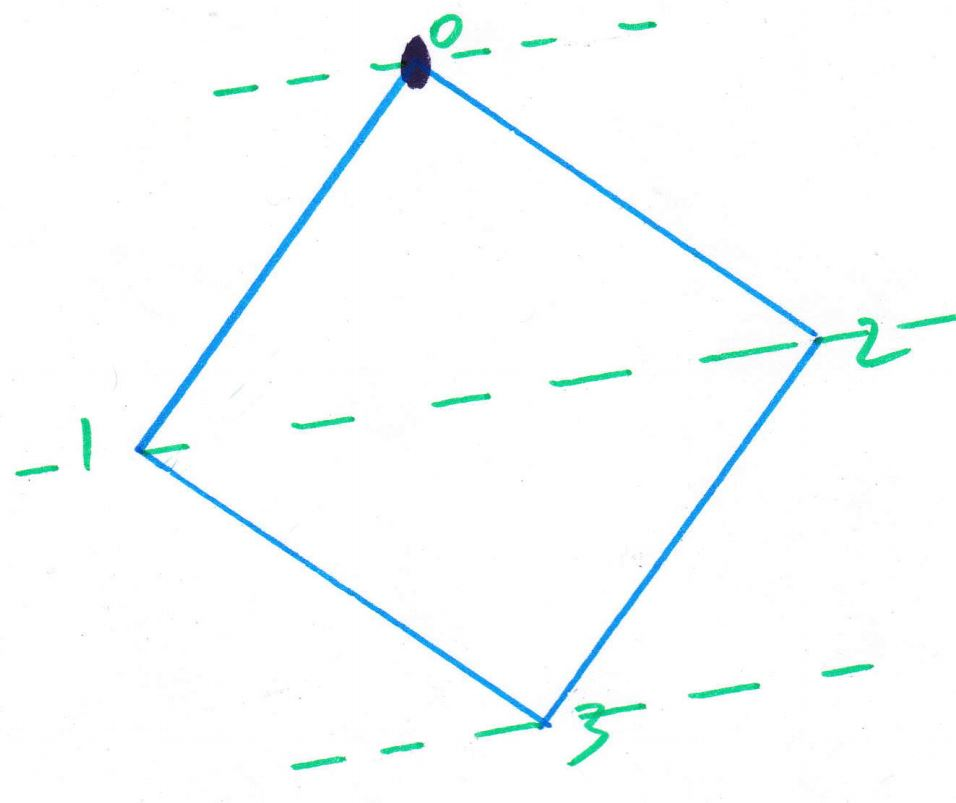
\includegraphics[width=0.5\columnwidth]{figure/2t2.JPG}
\caption{The 2*2 mesh network and the root processor is $P_{0}$}
\label{fig:2t2}
\end{figure}

The processor $P_{0}$, $P_{1}$ and $P_{2}$ start to process its respective fraction at the same time.  This includes $P_{1}$ and $P_{2}$ as they are relayed load in virtual cut-through mode at $t = 0$.  The processor $P_{3}$ starts to work when the $\alpha_{1}$ and $\alpha_{2}$ complete transmission.  That is, the link $0-1$ and $0-2$ are occupied 
transmitting load to processor $1$ and $2$, respectively and only transmission to $3$ when that is finished.
According to the divisible load theory  \cite{bharadwaj2003divisible}, we obtain the timing diagram Fig ~\ref{fig:2t2d}.  

\begin{figure}[!ht]
\centering
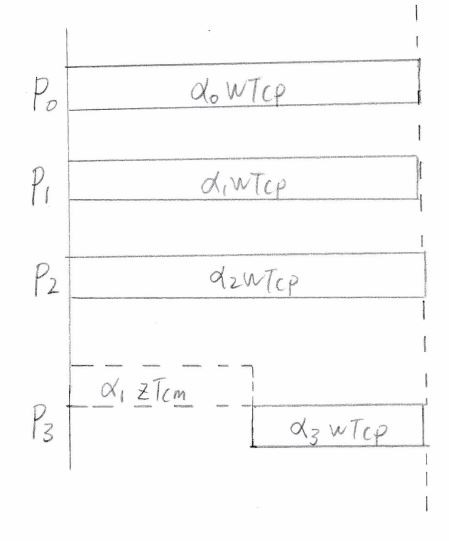
\includegraphics[width=0.5\columnwidth]{figure/2t2d.JPG}
\caption{The timing diagram for 2*2 mesh network and the root processor is $P_{0}$}
\label{fig:2t2d}
\end{figure}

Here in the Gantt-like timing diagram communication appears above each axis and computations appears below the each axis.  Let's assume that all processors stop computing at the same time in order to minimize the makespan  \cite{sohn1992optimal}.

Based on the timing diagram, we obtain a group of linear equations to find the fraction workload assigned to each processor $\alpha_{i}$ : 

\begin{empheq}[left=\empheqlbrace]
{align}
\alpha_{0} \omega T_{cp} = T_{f, m}\\
\alpha_{1} \omega T_{cp} = T_{f, m}\\
\alpha_{2} \omega T_{cp} = T_{f, m}\\
\alpha_{1}zT_{cm} + \alpha_{3}\omega T_{cp} = T_{f, m}\\
\alpha_{0} + \alpha_{1} + \alpha_{2} + \alpha_{3} = 1\\
\sigma = \frac{zT_{cm}}{\omega T_{cp}}\\
0 < \sigma < 1 \\
0 < \alpha_{0} \leq  1\\
0 \leq  \alpha_{1},  \alpha_{2},  \alpha_{3}  < 1
\end{empheq}
\\

The group of equations are represented by the matrix form:

\begin{equation}
{
\left[ \begin{array}{ccc}
1 & 2 & 1\\
1 & -1 & 0\\
0 & \sigma-1 & 1
\end{array} 
\right ]} \times \left[ \begin{array}{c}
\alpha_{0} \\
\alpha_{1} \\
\alpha_{3} 
\end{array} 
\right ] = \left[ \begin{array}{c}
1 \\
0 \\
0 
\end{array} 
\right ]
\end{equation}
The matrix is represented as $A \times \alpha = b$.  $A$ is named as the \textbf{\textit{flow matrix}}.
Here because of symmetry $\alpha_{1} = \alpha_{2}$, so $\alpha_{2}$ is not listed in the matrix equations.

Finally, the explicit solution is:
\begin{empheq}[left=\empheqlbrace]
{align}
\sigma = \frac{zT_{cm}}{\omega T_{cp}}\\
\alpha_{0} = \frac{1}{4- \sigma}\\
\alpha_{1} = \frac{1}{4- \sigma}\\
\alpha_{3} = \frac{1 - \sigma}{4- \sigma}
\end{empheq}
\\
The equations say that as $\sigma$ grows,  the value $\alpha_{3}$ drops.  In other words, as the communication capacity decreases, there is less data workload assigned to $P_{3}$.  Further, it means it will be economical to keep the load local on $P_{0}$ $P_{1}$ $P_{2}$ and not distribute it, to other processors.  

The equivalence inverse speed of a a single processor is $w_{eq}$, that can replace the original network as
$$T_{f,n} = 1*w_{eq}*T_{cp}$$
$$w_{eq} = \alpha_{0}*w$$
$$Speedup = \frac{T_{f, 0}}{T_{f, n}}= \frac{\omega T_{cp}}{\alpha_{0}\omega T_{cp}} = \frac{1}{\alpha_{0}} = 4- \sigma$$

\subsection{2*n mesh network}
The $2*n$ Fig ~\ref{fig:2t10} homogeneous mesh network processes load $L$ and $L$ originates $P_{0}$.  

\begin{figure}[!ht]
\centering
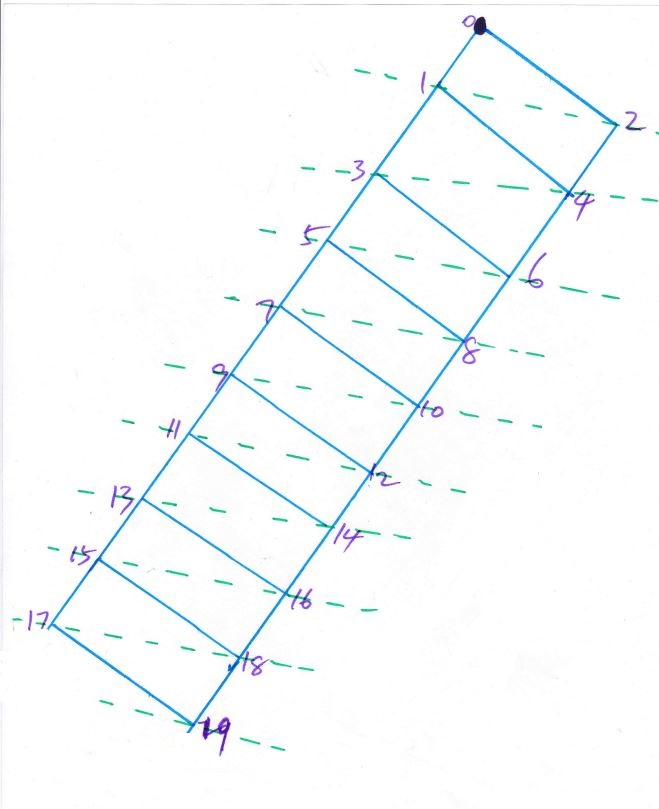
\includegraphics[width=0.6\columnwidth]{figure/2t10.JPG}
\caption{2*n (n = 10) mesh network and the workload happens on $P_{0}$}
\label{fig:2t10}
\end{figure}

Load a distribution from $P_{0}$ to $P_{1}$ and $P_{2}$ via virtual cut-through.  After $P_{1}$ and $P_{2}$ finish receiving load from link $0-1$ and $0-2$, they will be used to forward load to $P_{3}$ and $P_{4}$ and so on.

The equations are presented as:
\begin{empheq}[left=\empheqlbrace]{align}
\alpha_{0} \omega T_{cp} = T_{f, m}\\
\alpha_{1} \omega T_{cp} = T_{f, m}\\
\alpha_{2} \omega T_{cp} = T_{f, m}\\
\alpha_{1}zT_{cm} + \alpha_{3}\omega T_{cp} = T_{f, m}\\
\alpha_{2}zT_{cm} + \alpha_{4}\omega T_{cp} = T_{f, m}\\
(\alpha_{1} + \alpha_{3})zT_{cm} + \alpha_{5}\omega T_{cp} = T_{f, m}\\
\vdots \\
(\alpha_{1} \cdots + \alpha_{2 \times n - 1})zT_{cm} +\alpha_{2 \times n - 1} \omega T_{cp} = T_{f, m}\\
\alpha_{0} + \cdots + \alpha_{2 \times n - 1} = 1\\
\sigma = \frac{zT_{cm}}{\omega T_{cp}}\\
0 < \sigma < 1 \\
0 < \alpha_{0} \leq 1\\
0 \leq \quad \alpha_{1} \quad \alpha_{2} \quad  \cdots  \quad \alpha_{2 \times n - 1} < 1
\end{empheq}


The flow matrix closed-form is shown:
\begin{equation}
{
\left[ \begin{array}{ccccccc}
1 & 2 & 2 & \cdots & 2 & 2 & 1\\
1 & -1 & 0 & \cdots& 0 & 0 & 0\\
0 & \sigma-1 & 1 & \cdots & 0 & 0 & 0 \\
0 & \sigma-1 & \sigma & 1 & 0 & \cdots & 0 \\
0 & \sigma-1 & \sigma & \sigma & 1 & 0 & 0 \\
\vdots & \vdots & \vdots  &   \vdots & \ddots & \ddots\\
0 & \sigma-1 & \sigma & \cdots & \sigma & \sigma & 1
\end{array} 
\right ]} \times \left[ \begin{array}{c}
\alpha_{0} \\
\alpha_{1} \\
\alpha_{3} \\
\alpha_{5} \\
\vdots \\
\alpha_{2 \times n - 3}\\
\alpha_{2 \times n - 1}
\end{array} 
\right ] = \left[ \begin{array}{c}
1 \\
0 \\
0 \\
0 \\
\vdots \\
0 \\
0
\end{array} 
\right ]
\end{equation}

According to the \textbf{\textit{Cramer's rule}},the explicit solution for the group of equations is:
\begin{empheq}[left=\empheqlbrace]
{align}
\alpha_{i} = \left |\frac{\det A^{\star}_{i}}{\det A}\right |
\end{empheq}
where $A^{\star}_{i}$ is the matrix formed by replacing the $i$-th column of A by the column vector b.\\
Especially,
\begin{equation}
{
A^{\star}_{0} = \left[ \begin{array}{ccccccc}
1 & 2 & 2 & \cdots & 2 & 2 & 1\\
0 & -1 & 0 & \cdots& 0 & 0 & 0\\
0 & \sigma-1 & 1 & \cdots & 0 & 0 & 0 \\
0 & \sigma-1 & \sigma & 1 & 0 & \cdots & 0 \\
0 & \sigma-1 & \sigma & \sigma & 1 & 0 & 0 \\
\vdots & \vdots & \vdots  &   \vdots & \ddots & \ddots\\
0 & \sigma-1 & \sigma & \cdots & \sigma & \sigma & 1
\end{array} 
\right ]}
\end{equation}

$$\alpha_{0} = \left |\frac{\det A^{\star}_{0}}{\det A} \right |$$
$$\det A^{\star}_{0} = -1$$

The equivalence inverse processing speed :
$$T_{f,n} = 1*w_{eq}*T_{cp}$$
$$w_{eq} = \alpha_{0}*w$$

Finally, the speedup is:
$$Speedup = \frac{T_{f, 0}}{T_{f, n}}= \frac{\omega T_{cp}}{\alpha_{0}\omega T_{cp}} = \frac{1}{\alpha_{0}} =  \left|-\det A\right|$$.

In addition, we can extend the flow matrix pattern to $m*n$ mesh network.

%\subsection{m*n mesh network}
%Considering a general $m*n$ mesh network,  such as Fig ~\ref{fig:3t8}.  

\begin{figure}[!ht]
\centering
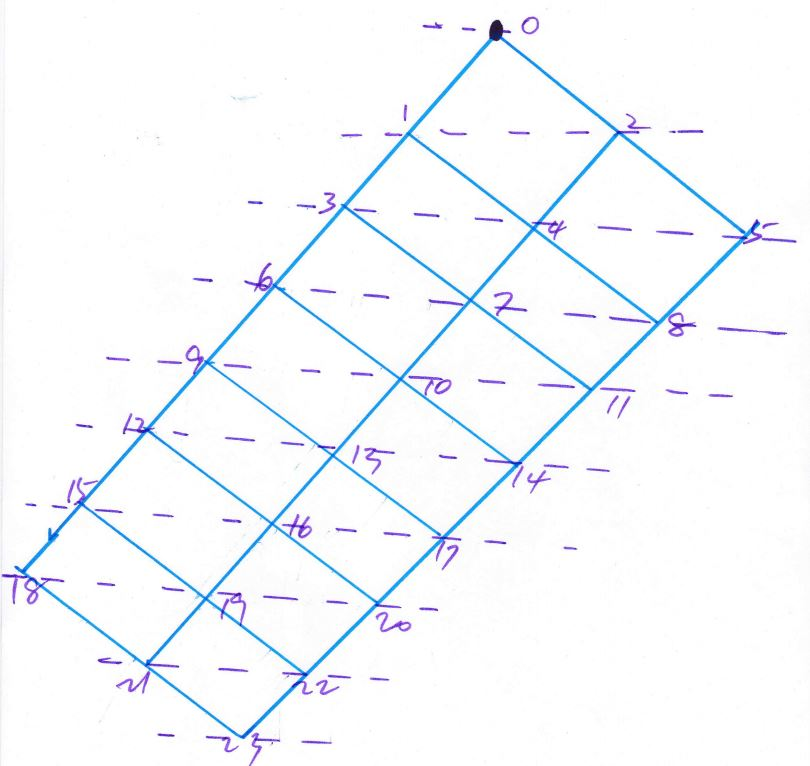
\includegraphics[width=0.55\columnwidth]{figure/3t8.JPG}
\caption{3*8 mesh network.  The data injection position is $P_{0}$}
\label{fig:3t8}
\end{figure}

Utilizing the previous methodology, we obtain the closed-form flow matrix equations for ~\ref{fig:3t8}:
\begin{equation}
{
\left[ \begin{array}{cccccccccc}
1 & 2 & 3 & 3 & 3 & 3 & 3 & 3 & 2 & 1\\
1 & -1 & 0 & 0 & 0 & 0 & 0 & 0 & 0 & 0\\
0 & \sigma-1 & 1 & 0 & 0 & 0 & 0 & 0 & 0 & 0 \\
0 & \sigma-1 & \sigma & 1 & 0 & 0 & 0 & 0 & 0 & 0 \\
0 & \sigma-1 & \sigma & \sigma & 1 & 0 & 0 & 0 & 0 & 0\\
0 & \sigma-1 & \sigma & \sigma & \sigma & 1 & 0 & 0 & 0 & 0\\
0 & \sigma-1 & \sigma & \sigma & \sigma & \sigma & 1 & 0 & 0 & 0\\
0 & \sigma-1 & \sigma & \sigma & \sigma & \sigma & \sigma & 1 & 0 & 0\\
0 & \sigma-1 & \sigma & \sigma & \sigma & \sigma & \sigma & \sigma & 1 & 0\\
0 & \sigma-1 & \sigma & \sigma & \sigma & \sigma & \sigma & \sigma & \sigma & 1 \\
\end{array} 
\right ]} \times \left[ \begin{array}{c}
\alpha_{0} \\
\alpha_{1} \\
\alpha_{3} \\
\alpha_{6} \\
\alpha_{9} \\
\alpha_{12}\\
\alpha_{15}\\
\alpha_{18}\\
\alpha_{21}\\
\alpha_{23}
\end{array} 
\right ] = \left[ \begin{array}{c}
1 \\
0 \\
0 \\
0 \\
0 \\
0 \\
0 \\
0 \\
\vdots \\
0
\end{array} 
\right ]
\end{equation}

We use the similar method to prove $\det A \neq 0$. 
The equivalence inverse processing speed :
$$T_{f,n} = 1*w_{eq}*T_{cp}$$
$$w_{eq} = \alpha_{0}*w$$

so the speedup is:
$$Speedup = \frac{T_{f, 0}}{T_{f, n}}= \frac{\omega T_{cp}}{\alpha_{0}\omega T_{cp}} = \frac{1}{\alpha_{0}} = \left |-\det A \right |$$.

The first row in flow matrix describe the number of cores on each $D_{i}$.
  For example, there is 1 core with $0$ hop distance ($D_{0}$) with load site $L$.  There are 2 cores with $1$ hop distance ($D_{1}$) with load site $L$.  There are 3 cores with $2$ hops distance ($D_{2}$) with load site $L$, and so on.
  
  The number of rows means the number of different type processor data fraction.  














\subsection{Proof of solution existence and unique}
We take $2*10$ mesh network as an example, other $m*n$ mesh network is proved by the same mathematics technique.

If the solution exist and is unique, we need to prove $\det A \neq 0$. 

\begin{equation}
{
C = \left[ \begin{array}{cccccc}
-1 & 0 & \cdots& 0 & 0 & 0\\
\sigma-1 & 1 & \cdots & 0 & 0 & 0 \\
\sigma-1 & \sigma & 1 & 0 & \cdots & 0 \\
\sigma-1 & \sigma & \sigma & 1 & 0 & 0 \\
\vdots & \vdots & \vdots  &   \vdots & \ddots & \ddots\\
\sigma-1 & \sigma & \cdots & \sigma & \sigma & 1
\end{array} 
\right ]
}
\end{equation}

$C$ is a lower triangular matrix and the diagonal elements are not $0$.  So $C$ is non-degenerate, that is, the matrix is column linear independence.

After a series of column reduction and row reduction actions, we get
\begin{equation*}
     {A = \left[ \begin{array}{ccccccc}
1 & 2 & 2 & \cdots & 2 & 2 & 1\\
1 & -1 & 0 & \cdots& 0 & 0 & 0\\
0 & \sigma-1 & 1 & \cdots & 0 & 0 & 0 \\
0 & \sigma-1 & \sigma & 1 & 0 & \cdots & 0 \\
0 & \sigma-1 & \sigma & \sigma & 1 & 0 & 0 \\
\vdots & \vdots & \vdots  &   \vdots & \ddots & \ddots\\
0 & \sigma-1 & \sigma & \cdots & \sigma & \sigma & 1
\end{array} 
\right ]}
\end{equation*}


\begin{equation*}
{
\xrightarrow[\text{Reduction}]{\text{Column}}\\
\left[ \begin{array}{ccccccc}
1 & 0 & 0 & \cdots & 0 & 0 & 0\\
1 & -3 & -2 & \cdots& -2 & -2 & -1\\
0 & \sigma-1 & 1 & \cdots & 0 & 0 & 0 \\
0 & \sigma-1 & \sigma & 1 & 0 & \cdots & 0 \\
0 & \sigma-1 & \sigma & \sigma & 1 & 0 & 0 \\
\vdots & \vdots & \vdots  &   \vdots & \ddots & \ddots\\
0 & \sigma-1 & \sigma & \cdots & \sigma & \sigma & 1
\end{array} 
\right ]}
\end{equation*}

\begin{equation*}
{\xrightarrow[\text{Reduction}]{\text{Row}}\\
\left[ \begin{array}{ccccccc}
1 & 0 & 0 & \cdots & 0 & 0 & 0\\
0 & -3 & -2 & \cdots& -2 & -2 & -1\\
0 & \sigma-1 & 1 & \cdots & 0 & 0 & 0 \\
0 & \sigma-1 & \sigma & 1 & 0 & \cdots & 0 \\
0 & \sigma-1 & \sigma & \sigma & 1 & 0 & 0 \\
\vdots & \vdots & \vdots  &   \vdots & \ddots & \ddots\\
0 & \sigma-1 & \sigma & \cdots & \sigma & \sigma & 1
\end{array} 
\right ]
}
\end{equation*}
Considering the matrix $\hat{C}$
\begin{equation}
{
\hat{C} = \left[ \begin{array}{cccccc}
-3 & -2 & \cdots& -2 & -2 & -1\\
\sigma-1 & 1 & \cdots & 0 & 0 & 0 \\
\sigma-1 & \sigma & 1 & 0 & \cdots & 0 \\
\sigma-1 & \sigma & \sigma & 1 & 0 & 0 \\
\vdots & \vdots & \vdots  &   \vdots & \ddots & \ddots\\
\sigma-1 & \sigma & \cdots & \sigma & \sigma & 1
\end{array} 
\right ]
}
\end{equation}
, which is still column linear independence.  Considering $0 < \sigma < 1$, the flow matrix is full rank. So $\det A \neq 0$.

After three user cases' investigation, we find a crucial methodology:
\textbf{$$\forall D_{i} = D_{j}, \quad then \quad \alpha_{i} = \alpha_{j},  \quad  0 \leq i,  j \leq m*n-1$$}

%\subsection{Sensitivity Analysis}
%The speedup is :
$$Speedup = \frac{T_{f, 0}}{T_{f, n}}= \frac{\omega T_{cp}}{\alpha_{0}\omega T_{cp}} = \frac{1}{\alpha_{0}} = \left |-\det A \right |$$.

\subsubsection{Data Injection On The Corner Processor}

One can see speedup increases with an increasing number of core (i.e. processor) and also increases with decreasing $\sigma$ (that is increasing communication speed relative to computation speed).

For a large number of cores and $\sigma$ close to one, speedup is three times. $P_{0}$ and two adjacent neighbor processor do most of the processing.


\subsubsection{Data Injection On The Boundary Processor}
The data injection happens on boundary processor $P_{2}$. 


Fig shows that if the value $\sigma > 0.2$, the speedup increases rapidly as a function of the number of cores.  If the value $\sigma < 0.1$, the number of cores has linear impact on the speedup performance.  If the number of cores is for $\sigma$ close to one, the speedup is about four since only the three processors close to $P_{0}$ and $P_{0}$ do almost all the processing.

\subsubsection{Data Injection On The Inner Grid Processor}
For a $5*n$ mesh network, $L$ originate on the inner grid $P_{12}$ and the simulation result says:



If the number of processor $ > 5$, the cluster equivalence computation ability is at least $5$ time speedup.  There are $5$ processors in the first stage.  For small $\sigma$ speedup growth is linear.  For large $\sigma$ and a large number of cores, speedup is about five as only $P_{0}$ and four adjacent processors do almost all the processing. 

\section{Multi-source Assignment Heuristic Algorithm}

\subsection{Equivalence Computation Algorithm}
If the data injection positions consist of a connected subgraph of $G$, we use $G_{L}$ to present it.

Our objective is to propose a general algorithm framework to minimize the makespan and give quantitative model analysis utilizing the flow matrix.  

The constraint comes from the divisible load theory linear equations.   

\title{LinearProgram}
\maketitle
\begin{alignat}{2}
\min\quad & T_{f,n}\\
\mbox{s.t.}\quad
&\sum_{i \in 0 \cdots (n-1)} \alpha_{i} = 1, &\quad& \\
&\alpha_{i} \geq 0, &{}& 
\end{alignat}

This algorithm is named as \textbf{\textit{Equivalence Processor Scheduling Algorithm (EPSA)}}.

\begin{algorithm}
\caption{Equivalence Processor Scheduling Algorithm (EPSA)}
\begin{algorithmic} 
\floatname{algorithm}{Procedure}
\renewcommand{\algorithmicrequire}{\textbf{Input:}}
\renewcommand{\algorithmicensure}{\textbf{Output:}}
\REQUIRE $k$ data injection positions
\ENSURE $m*n$ processor data fractions $\alpha_{i}$
\STATE Collapse the data injection processors into one ``big" equivalent processor  \cite{robertazzi1993processor}.
\STATE Calculate $m*n$ processor's $D_{i}$.
\STATE Obtain the flow matrix $A$.
\STATE Calculate $m*n$ processors data fraction $\alpha_{i}$.
\end{algorithmic}
\end{algorithm}

In term of the time complexity : 

\begin{itemize}
\item The time complexity of calculating the determinant is $O(r^{3})$ with Gaussian elimination or LU decomposition.  $r$ is the rank of flow matrix and $r$ is $O(\max(m,n))$.
\item The time complexity of calculating the flow matrix $A_{i}$ is $O(k*m*n)$. $k$ is the number of data injection.
\item The total time complexity is $O(k*\max(m,n)^{3})$.
\end{itemize}


\subsection{Intuitive Voronoi Division Algorithm}
Our objective is to propose an intuitive algorithm to minimize the makespan and give quantitative model analysis utilizing the flow matrix.  

Also, in each cell, the constraint comes from the divisible load theory linear equations.   

\title{LinearProgram}
\maketitle
\begin{alignat}{2}
\min\quad & T_{f,n}\\
\mbox{s.t.}\quad
&\sum_{i \in 0 \cdots (n-1)} \alpha_{i} = 1, &\quad& \\
&\alpha_{i} \geq 0, &{}&
\end{alignat}

The intuitive algorithm is named as \textbf{\textit{Manhattan Distance Voronoi Diagram Algorithm}}:
\begin{algorithm}
\caption{Manhattan Distance Voronoi Diagram Algorithm (MDVDA)}
\begin{algorithmic} 
\floatname{algorithm}{Procedure}
\renewcommand{\algorithmicrequire}{\textbf{Input:}}
\renewcommand{\algorithmicensure}{\textbf{Output:}}
\REQUIRE $k$ data injection positions
\ENSURE $m*n$ processor data fractions
\STATE Calculate $k$ Voronoi cells with Manhattan distance.
\STATE Calculate $k$ flow matrix $A_{i}$.
\STATE Display reduced Voronoi cells.
\STATE Illustrate reduced Voronoi cells' speedup curves.
\end{algorithmic}
\end{algorithm}

The time complexity of algorithm consists of two parts, one is about the determinant computation of flow matrix and the other is about the Manhattan distance Voronoi diagram. 




\subsection{Reduced Voronoi Division Algorithm}
After investigation, we find the makespan depends on the bottleneck makespan.  In other words, if other divisions own more processors than the bottleneck cell, it does not help to minimize the makespan.  

Our objective is to propose a heuristic algorithm to minimize the makespan and give quantitative model analysis utilizing the flow matrix.  In each cell, the constraint comes from the divisible load theory linear equations.   

The merits of new algorithm is finishing the task within the same makespan as MDVDA, yet utilizing less processors resource.

\title{LinearProgram}
\maketitle
\begin{alignat}{2}
\min\quad & T_{f,n}\\
\mbox{s.t.}\quad
&\sum_{i \in 0 \cdots n} \alpha_{i} = 1, &\quad& \\
&\alpha_{i} \geq 0, &{}& 
\end{alignat}


The heuristic algorithm is named as \textbf{\textit{Reduced Manhattan Distance Voronoi Diagram Algorithm}}:
\begin{algorithm}
\caption{Reduced Manhattan Distance Voronoi Diagram Algorithm (RMDVDA)}
\begin{algorithmic} 
\floatname{algorithm}{Procedure}
\renewcommand{\algorithmicrequire}{\textbf{Input:}}
\renewcommand{\algorithmicensure}{\textbf{Output:}}
\REQUIRE $k$ data injection positions
\ENSURE $m*n$ processor data fractions
\STATE Calculate $k$ Voronoi cells with Manhattan distance.
\STATE Calculate $k$ Voronoi cells' radius $R_{i}$.
\STATE Calculate $k$ flow matrix $A_{i}$.
\STATE $depth_{min} = \min ({Sp_{i}})$'s $R_{i}$.
\STATE Calculate the reduced Voronoi cells by setting the $depth_{i} = depth_{min}$ in each Voronoi cell.
\STATE Calculate reduced Voronoi cell's flow matrix $\hat{A_{i}}$.
\STATE Display reduced Voronoi cells.
\STATE Illustrate reduced Voronoi cells' speedup curves.
\end{algorithmic}
\end{algorithm}

In term of the time complexity :  
\begin{itemize}
\item The time complexity of Manhattan distance Voronoi cells is $O(k*m*n)$;
\item The time complexity of flow matrix determinant is $O(r^{3})$. $r$ is the rank of flow matrix.
\item So the total time complexity is $O(k*\max (m,n)^{3})$.
\end{itemize}

It displays that $10$ cells' equivalence computation is more balanced than the initial setting, and the whole cluster finishes processing load within the same time by less processors.
After $1000$ round random sampling experiments, we obtain the average saved processors ratio.

From the average saved processors ratio  , it shows the average percentage of saved processor is about $35 \%$.  


\subsection{Lower Band of Intuitive and Heuristic Algorithm}
Considering a $n*n$ mesh network, there are $l$ data load injections, the makespan is constrained by the makespan of bottleneck, so the best solution is each data load injection deploys data to its community, which is $\frac{n*n}{m}$ cores.  

For example, we calculate a $50*50$ mesh network and there are $l = 10$ load data injections.
Each node transmit data to $\frac{50*50}{10} = 250$ cores.  The first row of flow matrix in best situation is $row_{\mu}$ = [1     4     8    12    16    20    24   28  32  36  40  29];



\begin{itemize}
\item Sp : Speedup of an equivalence computation cell.
\item $optimal_{p}$ : practical optimal speedup of a load data injection, which is NP hard \cite{Liu_schedulingdivisible}
\item $optimal_{i}$ : optimal speedup of a load data injection in ideal situation
\item $\beta$ :  $\frac{Sp}{optimal_{i}}$ is the ratio between the speedup of an algorithm (i.e. EPSA or RMDVDA) over the practical ideal situation speedup.
\end{itemize}

According to the intuitive and heuristic algorithm, we can give a lower band of this algorithm.

$$\beta = \frac{Sp}{optimal_{i}} \leq \frac{Sp}{optimal_{p}}$$

$$Sp  \geq \beta * optiaml_{p}$$

We calculate the speedup of a community and the speedup of ideal situation.  In other words, we guarantee obtain a $\beta * optimal_{i}$ times approximation speedup of our algorithm.


\section{CONCLUSIONS}

\addtolength{\textheight}{-12cm}   % This command serves to balance the column lengths
                                  % on the last page of the document manually. It shortens
                                  % the textheight of the last page by a suitable amount.
                                  % This command does not take effect until the next page
                                  % so it should come on the page before the last. Make
                                  % sure that you do not shorten the textheight too much.

%%%%%%%%%%%%%%%%%%%%%%%%%%%%%%%%%%%%%%%%%%%%%%%%%%%%%%%%%%%%%%%%%%%%%%%%%%%%%%%%



%%%%%%%%%%%%%%%%%%%%%%%%%%%%%%%%%%%%%%%%%%%%%%%%%%%%%%%%%%%%%%%%%%%%%%%%%%%%%%%%



%%%%%%%%%%%%%%%%%%%%%%%%%%%%%%%%%%%%%%%%%%%%%%%%%%%%%%%%%%%%%%%%%%%%%%%%%%%%%%%%
\section*{APPENDIX}

\section*{ACKNOWLEDGMENT}

\printbibliography

\end{document}
